\documentclass{article}
\usepackage[en]{ukon-infie}
\usepackage[utf8]{inputenc}
\usepackage{algorithm2e}
\usepackage{amsmath}
\usepackage{graphicx}
% kann de oder en sein
% kann bubble break, topexercise sein

\Names{Jonas Probst, Simon Giebenhain, Gabriel Scheibler, Clemens Gutknecht}
\Lecture[DLCV]{Deep Learning for Computer Vision}
\Term{WS 2017/18}

\begin{document}
    \begin{ukon-infie}[28.1.18]{4}

		
		\begin{exercise}[p=20]{Transposed Convolutions}
		\question{}
		{
			One possible solution is:\\
			$x1=17, x2=15\\ x3=3, x4=2\\ x5=15, x6=13\\ x7=2, x8=6$
		}
		\question{}{}
		\begin{verbatim}
		
		
			W3 = tf.Variable(tf.zeros([3,3,15,13]))
			layer3 = tf.nn.conv2d_transpose(layer2, W3, output_shape=tf.constant(np.array([-1,22,24,15],
			dtype=np.int32)), strides=[1,2,6,1], padding = 'SAME')
			W4 = tf.Variable(tf.zeros([3,3,17,15]))
			layer4 = tf.nn.conv2d_transpose(layer3, W4, output_shape=tf.constant(np.array([-1,64,48,17],
			dtype=np.int32)), strides=[1,3,2,1], padding = 'SAME')
			layer4.shape
			TensorShape([Dimension(None), Dimension(64), Dimension(48), Dimension(17)])
		\end{verbatim}	
		
		\question{}
		{
			It's not clear how much padding was used in the convolution, so output shape needs to be specified in the method.
		}
		\end{exercise}
		
		\begin{exercise}[p=60]{Encoder-Decoder}
		\question{}
		{
		The method \textbf{normalize\_mean()} and \textbf{normalize\_stddev()} normalize the mean and standard deviation of the input data respectively.
		}
		\question{}
		{		
		The architecture of our encoder-decoder is described in the following:\\
		\textbf{Encoder}:\\
		The inputs are images of size $[28 , 28 , 1]$.\\
		We apply a strided convolution with kernel dimensions $[3,3,1,32]$ and strides $[1,2,2,1]$ followed by basically the same convolution with kernel dimensions $[3,3,32,64]$ and strides $[1,2,2,1]$. This yields an output of the following shape $[7,7,64]$.\\
		The last step of the encoder is a fully connected layer, which reduces the data to a vector of size 512.\\
		A dropout layer connects encoder and decoder.\\
		
		\textbf{Decoder:}\\
		First the data of shape $[\text{batch\_size},512 ]$ is transformed to shape $[\text{batch\_size},7,7,64 ]$ with a fully connected layer and reshaping.\\
		Afterwards we apply transposed convolutions mirroring the convolutions of the encoder, such that we come form shape $[7,7,64]$ to $[28,28,1]$ per image. An additional fully connected layer, which maintains shape, follows the convolutions.
		
		\textbf{Further Details:} \\
		We used \textit{parametric ReLU} as activation function and applied \textit{batch normalization} before every activation.\\
		As mentioned above we applied a \textit{droupout-layer} inbetween encoder and decoder.
		}
		\question{}
		{
		We struggled to come up with a sensible training method. At first we believed, that classifying(pretrained on the latin training dataset) the output of the encoder-decoder and apllying cross entropy to the result, would be the best idea. We followed this approach in \textbf{encoder\_decoder\_class.py}. We achieved quit solid results, with a classification accuracy of around 97\%. However, the outputs of the encoder-decoder were not readable for humans. This is due to the fact, that the classifier classifies every input he gets, and cannot distinguish between a nice letter and some extremly noisy letter. We tried to fix this, by introducing a noise class, with randomly generated training examples labeled as noise, but it did not help. \\
		Here is a visualization of the results:\\
		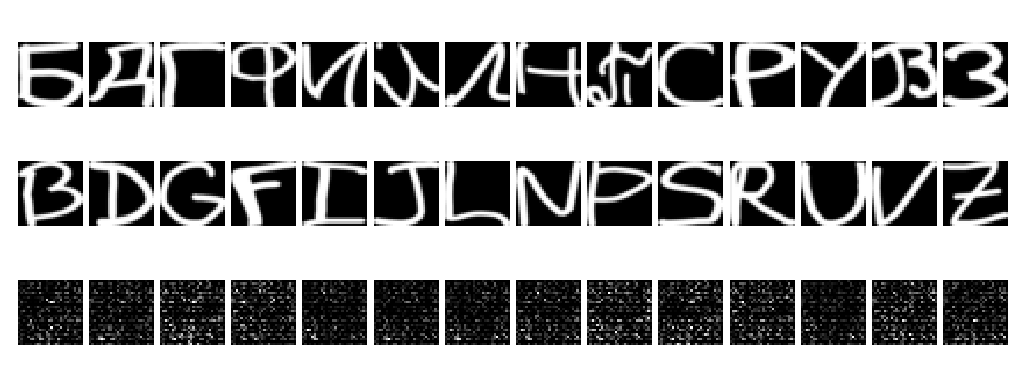
\includegraphics[scale=0.5]{encoder_decoder_class.png}
		
		
		Another approach for the loss function, is to take the L2-loss of the output of the encoder-decoder with random examples of latin letters of the same class. This approach seemed to work quite well. However the outputs are always very similar within each class.\\
		
		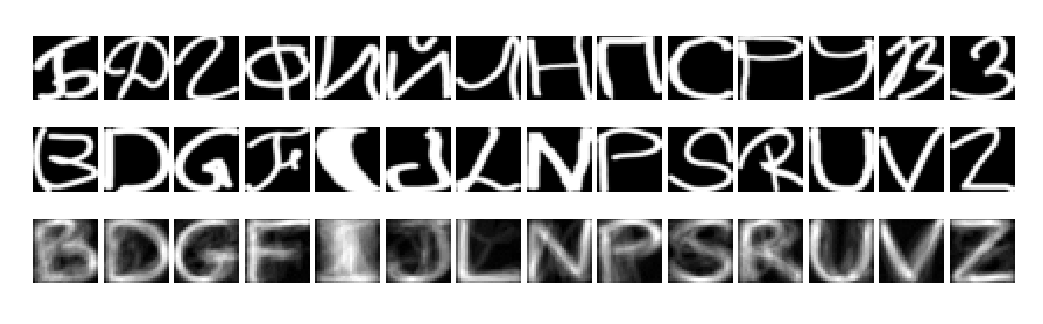
\includegraphics[scale=0.5]{encoder_decoder_random.png}
		
		One could also choose a representative for each class of the latin latters and always compute the L2-loss of the difference of the output of the encoder-decoder and the respective representative. This basically achieves, that for every cyrillic letter of class $k$ the encoder-decoder outputs the representativ of class $k$. (The same could be achieved with simple classification and return the representative of that class)\\
		Here is a visualization:\\
		
		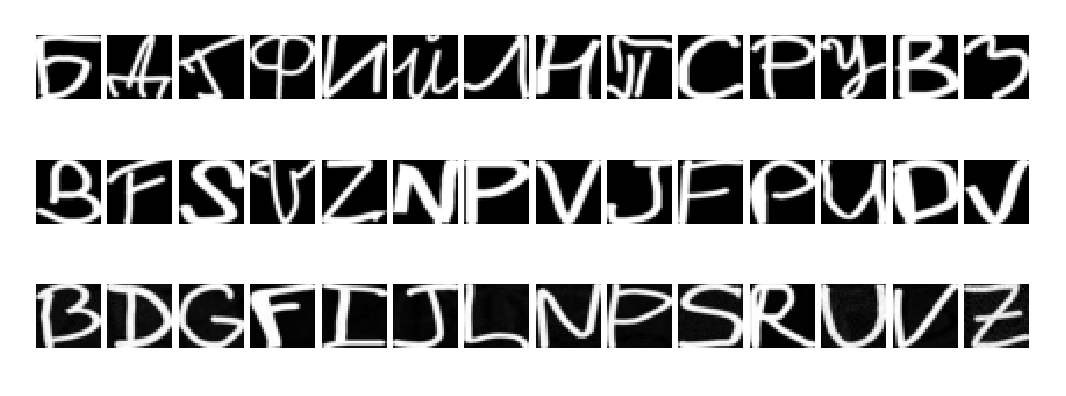
\includegraphics[scale=0.5]{encoder_decoder_single.png}

		
		
		Also one could always compare with the mean of the respective class, which does not really make sense, because the network is then trained to basically classify the image and return the mean of the resulting class. Here are the results:\\
		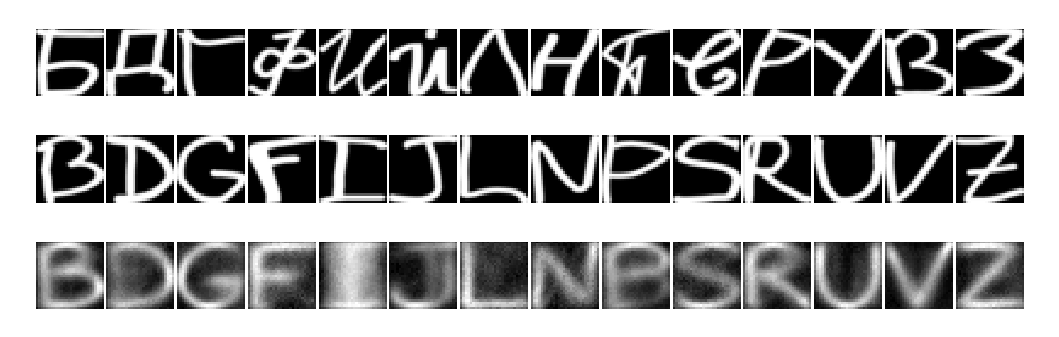
\includegraphics[scale=0.5]{decoder_encoder_mean.png}
		
		\textbf{Tricks:} Mentioned above in (b)
		
		}
		\question{}
		{
		See (c).
		}
		\question{}
		{
		For this exercise we used the training strategy and weights of \textbf{encoder\_decoder\_random.py}. The script \textbf{latent\_space.py} loades the weights saved in \textbf{encoder\_decoder\_random.train\_for\_latent\_space()}. The encoder part of the network is obmitted, it begins with the 512-tupel, which was in the middle before. All variables are markes as untrainable and only the 512-tupel is trainable. We optimezed for every class, the loss for a single class is the MSE of the output of the encoder and all training examples of that class. The results are shown below:\\
		
		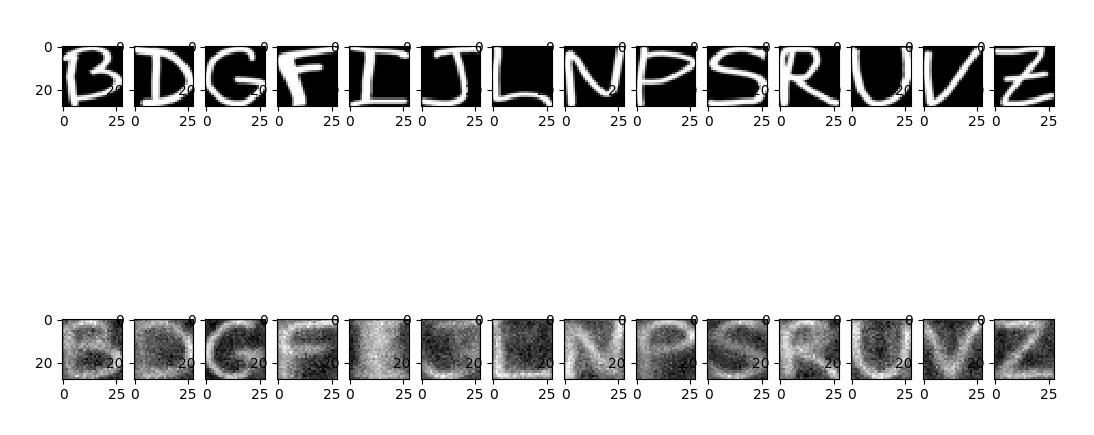
\includegraphics[scale=0.5]{latent_space.png}
		}
		
		\end{exercise}
		
		\begin{exercise}[p=10]{Backpropagation trough a ConvLayer}
		\question{}
		{
		We can interpret $A$ as a function $F_A: \mathbb{R}^n \rightarrow \mathbb{R}^m, x \mapsto Ax$
		Applying the multidimensional chain rule on $E(x) = g(Ax) = g(F_A(x))$ yields:\\
		$$D_xE(x) = D_xg(F_A(x)) \cdot D_xF_A(x)$$
		With the fact that $D_xE(x) = \nabla E(x)^T$, we get:\\
		$$\nabla E(x) = (D_xg(F_A(x)) \cdot D_xF_A(x))^T = (\nabla g(F_A(x))^T \cdot A)^T = A^T \cdot \nabla g(F_A(x))$$
		}
		\question{}
		{
			This can be nicely explained with (a). We could interpret $E$ as our loss, $g$ as our activation function and $A$ as a convolution (in the lecture we discussed that every convolution can be expressed with a matrix). If we want to apply some form of gradient descent, we have to compute the gradient of $E$, which is done using backpropagation. As we saw in (a) the gradient of $E$ depends on $\nabla g$ and $A^T$. And from the lecture we know, that $A^T$ is the transposed convolution to $A$ (this is where the name comes from).
		}
		
		\end{exercise}
		\begin{exercise}[p=20]{PCA vs. Auto-Encoder}
		\question{}
		{
		Let $x \in \mathbb{R}^d$. Let$v_1, \dots , v_d$ be the $d$ principal components, and $\tilde{V} := (v_1, \dots, v_k)$ be the matric with the first $k$ principal components.\\
		The projection is done, in the following way: First the length of the projection of $x$  onto each $v_i$ is calculated by the dot product: $v_i^T x$, then $v_i$ is scaled by this factor. Then all resulting vectors are combined to represent $x$ in the k dimensional subspace. In compact form:\\
		$$ \sum_{i=1}^k (v_i^T x)v_i = (\tilde{V}\tilde{V}^Tx) \in \mathbb{R}^d$$
		}
		\question{}
		{
			For this we make the assumption, that the data has zero mean, that is: $\frac{1}{L}\sum_{l=1}^L x_l = 0$ (otherwise one would first have to shift the data to achieve zero mean.)\\
			
			The loss for the auto-encoder is the following:\\
			$$ \sum_{l=1}^L \Vert x - BAx\Vert_2^2$$
			
			In terms of the PCA $A = \tilde{V}^T$ and $B= \tilde{V}$.
			Before we simplify this expression, two remarks:\\
			\begin{equation}
			v_i^Tv_i = 1 \qquad (\text{for all } i)
			\end{equation}
			\begin{equation}
			v_i^Tv_j = 0 \qquad (\text{for all } i\not= j)
			\end{equation}
			Both follow, because the principal components are a orthonormal basis.\\
			
			Furthermore x can be represented exactly, if all principal components are used(because they form a orthonormal basis), that is:\\
			\begin{equation}
			x= \sum_{i_1}^d (v_i^T x)v_i
			\end{equation} 
			and note the definition of the covariance matrix $\Sigma$
			\begin{equation}
			\Sigma := \frac{1}{L} \sum_{i=1}^L(x_i - \overline{x})(x_i-\overline{x})^L \stackrel{zero mean}{=} \frac{1}{L} \sum_{i=1}^Lx_ix^L
			\end{equation}
			
			There we can express the l2-loss in the following way:
			
			\begin{eqnarray}
			\sum_{l=1}^L \Vert x - \tilde{V}\tilde{V}x_l \Vert_2^2
			&\stackrel{(3)}{=}& \sum_{l=1}^L \Vert (\sum_{i=1}^d (v_i^T x_l)v_i) - (\sum_{i=1}^k (v_i^T x_l)v_i) \Vert_2^2 \\
			&=& \sum_{l=1}^L \Vert \sum_{i=k+1}^d (v_i^T x_l)v_i \Vert_2^2 \\
			&=& \sum_{l=1}^L \left(\sum_{i=k+1}^d (v_i^T x_l)v_i)\right)^T \left(\sum_{i=k+1}^d (v_i^T x_l)v_i)\right) \\
			&=& \sum_{l=1}^L \left(\sum_{i=k+1}^d (v_i^T x_l)v_i^T\right) \left(\sum_{i=k+1}^d (v_i^T x_l)v_i)\right) \\
			&=& \sum_{l=1}^L \left(\sum_{i=k+1}^d \sum_{j=k+1}^d (v_i^T x_l)^2v_i^Tv_j)\right) \\
			&=& \sum_{l=1}^L \left(\sum_{i=k+1}^d(v_i^T x_l)^2v_i^Tv_i + \sum_{i=k+1}^d \sum_{i\not=j=k+1}^d (v_i^T x_l)^2v_i^Tv_j\right) \\
			&\stackrel{(2)}{=}& \sum_{l=1}^L \left(\sum_{i=k+1}^d(v_i^T x_l)^2v_i^Tv_i \right) \\
			&\stackrel{(1)}{=}& \sum_{l=1}^L \left(\sum_{i=k+1}^d(v_i^T x_l)^2 \right) \\
			&=& \sum_{i=k+1}^d\left(\sum_{l=1}^L(v_i^T x_l)(v_i^T x_l) \right) \\
			&=& \sum_{i=k+1}^d\left(\sum_{l=1}^L(v_i^T x_l)(x_l^Tv_i) \right) \\
			&\stackrel{(4)}{=}& L \cdot \sum_{i=k+1}^dv_i^T \Sigma v_i\\
			&=& L \cdot \sum_{i=k+1}^dv_i^T \lambda_i v_i\\
			&\stackrel{(1)}{=}& L \cdot \sum_{i=k+1}^d\lambda_i\\
			\end{eqnarray}						
			
			Now we still have to prove, that $\tilde{V}$ is indeed a minimizer for $ \sum_{l=1}^L \Vert x - WW^Tx\Vert_2^2$.\\
			For this we continue by minimizing (15)	with respect to $v_{k+1}, \dots , v_{d}$ under the condition, that $v_i^Tv_i = 1$ and $v_i^Tv_j = 0$ for every $i \not = j$.\\
			
			The Lagragian is:\\
			$$F(\tilde{V}, \lambda) = \sum_{i=k+1}^dv_i \Sigma v_i + \sum_{i=k+1}^d \lambda_i (1- v_i^Tv_i) + \sum_{i=k+1}^d \sum_{i\not=j=k+1}^d \lambda_{i,j}v_i^Tv_j$$.
			Setting the deriviative to zero yields:\\
			$$ \frac{\partial F(\tilde{V}, \lambda)}{\partial v_i} = 2 \Sigma v_i - 2 \lambda_i v_i + \sum_{i\not=j=k+1}^d \lambda_{i,j}v_j \stackrel{!}{=}0$$
			When multiplying with $v_j$ ($j \not=i$), one sees, that $\lambda_{i,j}$ has to be zero(beacuse of the conditions (1) and (2)):\\
			$v_j \frac{\partial F(\tilde{V}, \lambda)}{\partial v_i} = \lambda_{i,j} \stackrel{!}{=}0$.\\
			
			What remains is the following:\\
			$$\frac{\partial F(\tilde{V}, \lambda)}{\partial v_i} != 0 \Leftrightarrow \Sigma v_i = \lambda_i v_i$$
			
			Therefore, we know that $\tilde{V}$ has to only consist out of eigenvectors of the covariance matrix. But which ones?\\
			We already know that the error is  $L \cdot \sum_{i=k+1}^d\lambda_i$. From this, it immediately follows, that for $v_{k+1}, \dots, v_{d}$ the eigenvectors with the smalles eigenvalues have to be chosen.\\
			
			In a nutshell:\\
			
			The reconstruction error of the PCA is minimal, if we choose the $k$ eigenvectors with the biggest eigenvalues to construct $\tilde{V}$, then the following holda for the reconstruction error:\\
			$$\sum_{l=1}^L \Vert x - \tilde{V}\tilde{V}x_l \Vert_2^2 = L \cdot \sum_{i=k+1}^d\lambda_i$$ \\
			, where $\lambda_{k+1}, \dots, \lambda{d}$ are the smalles eigenvalues of the covariance matrix of our training data.
		}
		\question{}
		{
			When utilizing SGD, still the equation from above holds ($B$ is the batch size): \\
			$$\sum_{l=1}^B \Vert x - \tilde{V}\tilde{V}x_l \Vert_2^2 = (B-1) \cdot \sum_{i=k+1}^dv_i^T \hat{\Sigma} v_i$$
			
			However, this time we only have an estimate of the the covariance matrix $\hat{\Sigma}$. \\
			Here $\hat{\Sigma} = \frac{1}{B-1} \sum_{i=1}^B(x- \overline{x})(x-\overline{x})^T$. This estimator is at least unbiased, but for small $B$ the training will sigificantly suffer. For bigger $B$ the there shouldn't be a noticable performance loss.
		}
		
		\end{exercise}

\end{ukon-infie}
\end{document}
